%start preamble
\documentclass[paper=a4,fontsize=11pt]{scrartcl}%kind of doc, font size, paper size

\usepackage{fontspec}
\defaultfontfeatures{Ligatures=TeX}
%\setsansfont{Liberation Sans}
\usepackage{polyglossia}	
\setdefaultlanguage[spelling=new, babelshorthands=true]{german}

\usepackage{amsmath}%get math done
\usepackage{amsthm}%get theorems and proofs done
\usepackage{graphicx}%get pictures & graphics done
\graphicspath{{pictures/}}%folder to stash all kind of pictures etc
\usepackage{amssymb}%symbolics for math
\usepackage{amsfonts}%extra fonts
\usepackage{caption}%captions under everything
\usepackage{listings}
\usepackage[titletoc]{appendix}
\numberwithin{equation}{section} 
\usepackage{float}%for garphics and how to let them floating around in the doc
\usepackage{wrapfig}%making graphics floated by text and not done by minipage
\usepackage{hyperref}
\usepackage{fancyhdr}
\usepackage{xcolor}%nicer colors, here used for links
\usepackage{csquotes}
\usepackage{enumitem}

\usepackage[backend=biber,style=alphabetic,
citestyle=alphabetic]{biblatex} %biblatex mit biber laden
\addbibresource{sources.bib}

%settings colors for links
\hypersetup{
    colorlinks,
    linkcolor={blue!50!black},
    citecolor={blue},
    urlcolor={blue!80!black}
}

\definecolor{pblue}{rgb}{0.13,0.13,1}
\definecolor{pgreen}{rgb}{0,0.5,0}
\definecolor{pred}{rgb}{0.9,0,0}
\definecolor{pgrey}{rgb}{0.46,0.45,0.48}

%Header & Footers
\pagestyle{fancy}
\lhead{Netzwerke -- Übung\\Sommersemester 2021}
\rhead{FB 4 -- Angewandte Informatik\\Hochschule für Technik und Wirtschft Berlin}
\lfoot{Übungsblatt 04 -- Routing \& Traffic Analysis}
\cfoot{}
\fancyfoot[R]{\thepage}
\renewcommand{\headrulewidth}{0.4pt}
\renewcommand{\footrulewidth}{0.4pt}

\lstdefinestyle{Bash}{
  language=bash,
  showstringspaces=false,
  basicstyle=\small\sffamily,
  numbers=left,
  numberstyle=\tiny,
  numbersep=5pt,
  frame=trlb,
  columns=fullflexible,
  backgroundcolor=\color{gray!20},
  linewidth=0.9\linewidth,
  %xleftmargin=0.5\linewidth
}

%%here begins the actual document%%
\newcommand{\horrule}[1]{\rule{\linewidth}{#1}} % Create horizontal rule command with 1 argument of height

\DeclareMathOperator{\id}{id}

\begin{document}
\begin{center}
\Large{\textbf{Übungsblatt 4 -- Routing \& Traffic Analysis}}
\end{center}

\begin{center}\Large{\textbf{Aufgabe A -- Wiederholung: OSI-Modell \& Transport Layer + IP}}\end{center}\vskip0.25in
Dieser Aufgabenteil dient der Wiederholung der Vorlesung \footnote{Das heißt, wenn sie fit sind einfach überspringen. Kann aber auch als Klausurvorbereitung dienen.}
\begin{enumerate}
	\item Erläutern sie was in Netzwerken unter Datenkapselung verstanden wird.
	\item Schauen Sie folgendes Video: \url{https://youtu.be/iDCi_CJAyXs} (Transport Layer)
	\item Recherchieren Sie die Funktion, sowie den Aufbau des \emph{TCP}-Protokolls.\\
	\url{https://youtu.be/_WP9be9W3xE}
	\item Lesen sie \cite[Kap. 3.1, 3.4]{Kurose2012}
	\begin{enumerate}
		\item Auf welcher Ebene im OSI-Modell arbeitet \emph{TCP}?
		\item Welche Aufgabe übernimmt das oben genannte Protokoll?
		\item Aus welchen Segmenten besteht ein \emph{TCP}-Datagram?
		\item Zeigen Sie beispielhaft den Aufbau eines \emph{TCP}-Datagram.
	\end{enumerate}
	\item Recherchieren Sie die Funktion, sowie den Aufbau des \emph{UDP}-Protokolls.\\
	\url{https://youtu.be/xWsD6a3KsAI}
	\item Lesen sie \cite[Kap. 3.3]{Kurose2012}
	\begin{enumerate}
		\item Auf welcher Ebene im OSI-Modell arbeitet \emph{UDP}?
		\item Welche Aufgabe übernimmt das oben genannte Protokoll?
		\item Aus welchen Segmenten besteht ein \emph{UDP}-Datagram?
		\item Zeigen Sie beispielhaft den Aufbau eines \emph{UDP}-Datagram.
	\end{enumerate}
	\item Worin unterscheiden sich \emph{TCP} und \emph{UDP} grundlegend?
	\item Recherchieren Sie die Funktion, sowie den Aufbau des IP-Protokolls.
	\item Lesen sie \cite[Kap. 4.1]{Kurose2012}
	\begin{enumerate}
		\item Auf welcher Ebene im OSI-Modell arbeitet IP?
		\item Welche Aufgabe übernimmt das oben genannte Protokoll?
		\item Aus welchen Segmenten besteht ein IP-Paket im allgemeinen?
	\end{enumerate}
	\item Recherchieren Sie die Funktion, sowie den Aufbau von Ethernet (\emph{IEEE 802.3} Protokollfamilie).
	\item Lesen sie \cite[Kap. 5ff]{Kurose2012}
	\begin{enumerate}
		\item Auf welcher Ebene im OSI-Modell arbeitet \emph{Ethernet}?
		\item Welche Aufgabe übernimmt das oben genannte Protokoll?
		\item Aus welchen Segmenten besteht ein Ethernet-Frame?
	\end{enumerate}
\end{enumerate}

\begin{center}\Large{\textbf{Aufgabe B -- TCP: 3-Way-Handshake}}\end{center}\vskip0.2in
Da TCP ein verbindungsorientiertes Protokoll ist, ist der Aufbau eines Sockets etwas komplizierter. Beide Seiten müssen sichergehen, dass die Verbindung korrekt funktioniert.
\begin{enumerate}
	\item Recherchieren Sie wie der 3-Way-Handshake bei TCP funktioniert \cite[Kap. 3.5]{Kurose2012}
	\item Gegeben sei Folgendes Sequenzdiagramm einer TCP Verbindung.
	\begin{figure}[H]
		\centering
		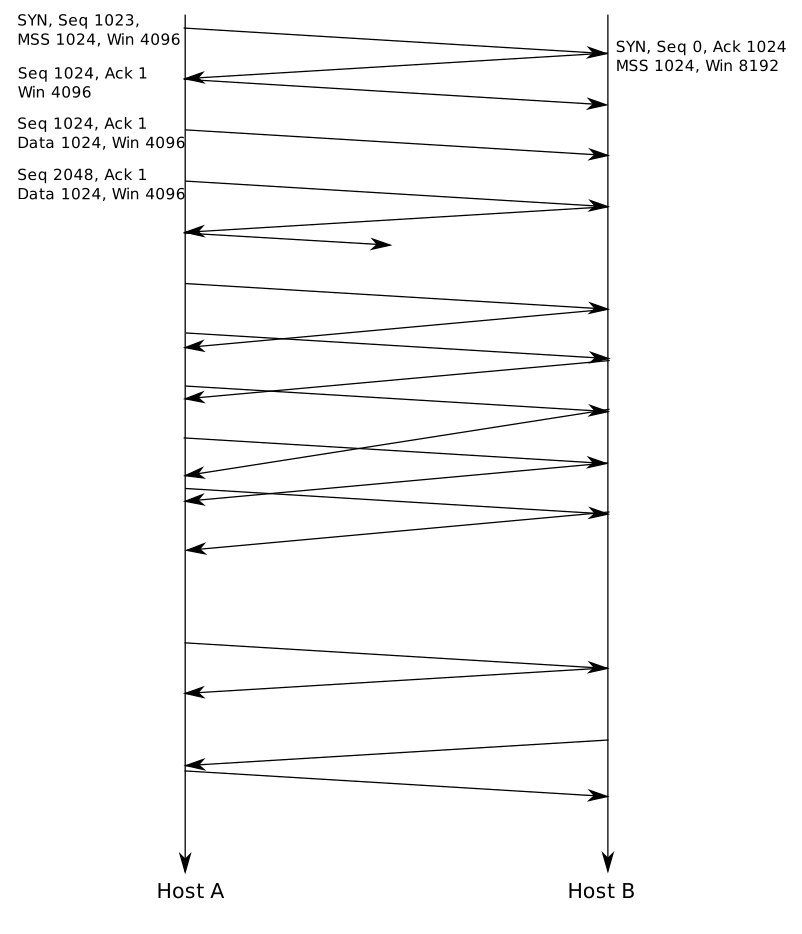
\includegraphics[scale=0.3]{handshake}
	\end{figure}
	Die horizontalen Pfeile repräsentieren die Zeit. Die Beschriftungen sollen die Header-Felder der TCP-Segmente beschreiben. Eine 3-Way-Handshake wird von Host A initialisiert.
	\item Erläutern sie den Austausch der ersten drei Segmente und Werte der Header-Felder.
	\item Host $A$ übermittelt 7 Segmente mit einer Nutzlast (Payload) von 1024 Byte an Host $B$, anschließend schließt $A$ die Verbindung. Die ersten beiden Segmente samt Nutzdaten sind im Sequenzdiagramm bereits beschriftet. Vervollständigen Sie die restlichen Segmente samt Werte anhand folgender Informationen:
	\begin{itemize}
		\item[a)] Eines der Segmente ging verloren (signalisiert durch eine Pfeil der nicht die rechte Seite erreicht)
		\item[b)] Nehmen sie an, das Host $A$ den Fast-Retransmit unterstützt und keine Timeouts durch ein verlorenes Segment auftritt.
	\end{itemize}
\end{enumerate}

\begin{center}\Large{\textbf{Aufgabe C -- Wiederholung: ICMP}}\end{center}\vskip0.2in
Bevor es zum Thema Routing geht, soll im Folgenden noch das ICM-Protokoll betrachtet werden. Dieses dient in vielen Fällen als Diagnoseprotokoll.
\begin{enumerate}
	\item Lesen sie den Abschnitt 4.4.3 zu ICMP \cite[S. 353]{Kurose2012}. 
	\item Was ist die Funktion des Internet Control Message Protocol (ICMP)?
	\item ICMP hat verschiedene Message-Codes (einige brauchen wir in den Übungen 4 und 5!). Erläutern sie was diese Nachrichten kodieren sollen -- was ist der Zweck der Message-Codes?
	\item Recherchieren sie welchen Hinweis Ihnen die verschiedenen \emph{ICMP}-Messages geben.
		\begin{itemize}
			\item[i)] Echo
			\item[ii)] Echo Reply
		\end{itemize}
\end{enumerate}

\begin{center}\Large{\textbf{Aufgabe D -- Wiederholung: Routing-Algorithmen}}\end{center}\vskip0.2in
\begin{enumerate}
	\item In der Vorlesung haben sie zwei Routing-Algorithmen kennen gelernt. Dies sind das Distanz-Vektor- und Link-State-Routing. Beide ermöglichen es den kürzesten Weg durch einen Graphen zu finden (Shortest-Path-Problem).\\
	Für gewöhnlich wird für das Distanz-Vektor-Routing der Bellman-Ford-Algorithmus verwandt, das Link-State-Routing nutzt den Dijkstra-Algorithmus. \cite[S. 363ff]{Kurose2012}
	\begin{enumerate}
		\item Recherchieren sie wie das Link-State-Routing unter Nutzung des Dijkstra-Algorithmus funktioniert \cite[S. 366]{Kurose2012}.
		\item Recherchieren sie wie das Distanz-Vektor-Routing unter Nutzung des Bellman-Ford-Algorithmus funktioniert  \cite[S. 371]{Kurose2012}.
		\item In welchen Protokollen finden diese beiden Protokollen Verwendung? Ist diesen Protokollen etwas gemein?
		\item Erläutern sie die fundamentalen Unterschiede beider Lösungsansätze.
		\item Warum wird keines der beiden Verfahren für das Exterior-Gateway-Protokoll genutzt?
		\item Diskutieren sie, ob der Bellman-Ford-Algorithmus für das Link-State-Routing und der Dijkstra-Algorithmus für das Distanz-Vektor-Routing genutzt werden könnte.
	\end{enumerate}
	\item Gegeben sei folgender Graph:
	\begin{figure}[H]
		\centering
		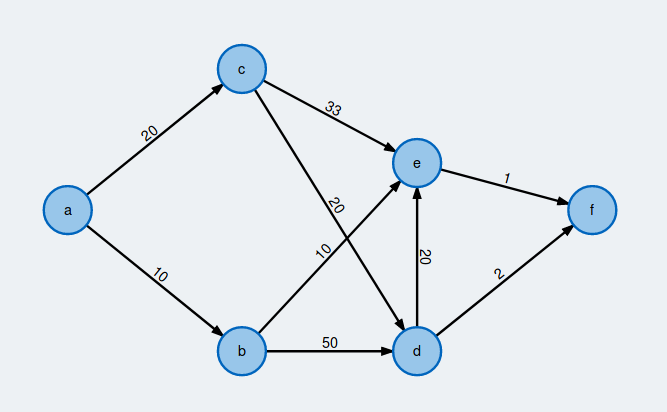
\includegraphics[scale=0.4]{dijkstra_example}
	\end{figure}
	Finden sie den kürzesten Weg vom Knoten $a$ zum Knoten $f$!
	\begin{enumerate}
		\item Nutzen sie zunächst den Dijkstra-Algorithmus.
		\item Nutzen sie den Bellman-Ford-Algorithmus.
	\end{enumerate}
\end{enumerate}

\begin{center}\Large{\textbf{Aufgabe E -- Traceroute}}\end{center}\vskip0.2in
\begin{enumerate}
	\item Lesen sie die folgenden Artikel:\\
	\url{https://en.wikipedia.org/wiki/Traceroute},\\
	\url{https://linux.die.net/man/8/traceroute}.\\
	Beantworten sie anschließend folgende Fragen:
	\begin{enumerate}
		\item Wofür wird Traceroute genutzt?
		\item Wie wird Traceroute umgesetzt, d.h. wie läuft eine Routen-Verfolgung ab? 
		\item Welche ICMP-Messages werden für die Realisierung genutzt?
		\item Welche Limitationen ergeben sich aus dieser Umsetzung?
		\item Dokumentieren sie die Syntax, sowie die Bedeutung von Traceroute beispielhaft.
	\end{enumerate}
	\item Lesen sie folgendes Paper zu Paris-Traceroute \cite{Augustin2006ATA} von der ACM International Measurement Conference (IMC) 2006:\\
	\url{http://conferences.sigcomm.org/imc/2006/papers/p15-augustin.pdf}
	\begin{enumerate}
		\item Warum ist eine \enquote{neue} Traceroute-Applikation notwendig?
		\item Nennen sie drei Topologie-Anomalien die durch Paris-Traceroute erkannt werden kann.
		\item Recherchieren sie wie \emph{paris-traceroute} zu nutzen ist! Notieren sie sich entsprechend die Kommandos und deren Bedeutung.
	\end{enumerate}
\end{enumerate}	

\begin{center}\Large{\textbf{Aufgabe F -- Wireshark}}\end{center}\vskip0.25in
Wireshark ist eine Open-Source-Software, mit dem Analysen, Fehlerbehebungen, Software- und Protokollkommunikation untersucht werden können. \emph{Wireshark} ähnelt \emph{tcpdump} in gewisser Weise, jedoch bietet \emph{Wireshark} ein grafisches Frontend (GUI), sodass die Analysen visuell ansprechend dargestellt werden können.\footnote{Wireshark kann natürlich auch als \emph{CLI} genutzt werden.}
\begin{enumerate}
	\item Lesen Sie folgendes Tutorial in Hinblick auf die Fragen in Aufgabenteil 3.): \url{https://www.howtogeek.com/104278/how-to-use-wireshark-to-capture-filter-and-inspect-packets/}
	, alternativ gibt es ein Wireshark 101 unter: \url{https://youtu.be/f4zqMDzXt6k} 
	\footnote{Lohnenswert ist das Wireshark 101 Buch im PDF Format (eine Suche bei Google hilft bestimmt).}
	\item Nachdem Sie die Tutorials abgearbeitet haben:
	\begin{enumerate}
		\item Was ist ein \emph{Network-Sniffer}?
		\item Wozu kann ein Netzwerk-Sniffer genutzt werden?
		\item Recherchieren sie wozu Filter in \emph{Wireshark} eingesetzt werden.
		\item Bringen sie in Erfahrung wie Filter genutzt werden.
		\item Welche beiden unterschiedlichen Mitschnitt-Modi (Caputre Modes) bietet \emph{Wireshark}? Worin unterscheiden sich diese?
	\end{enumerate}
	\item Erläutern sie anhand von Beispielen den grundlegende Umgang mit \emph{Wireshark}.
	\begin{enumerate}
		\item Wie stellen Sie Netzwerkinterfaces ein -- auf welchem Interface soll der Mitschnitt laufen.
		\item Wie filtern Sie nach Protokollen?
		\item Wie filtern Sie \emph{MAC}-Adressen?
		\item Wie filtern Sie \emph{IP}-Adressen?
	\end{enumerate}
\end{enumerate}

\begin{center}\Large{\textbf{Aufgabe G -- Wiederholung: Address Resolution Protocol (ARP) \& Neighbor Discovery Protocol (NDP)}}\end{center}\vskip0.25in
Es sollte ihnen aufgefallen sein, dass in der zweiten Übung (Geswitchte Netze) ihr Netzwerk in der Planung zwar IP-Adressen nutzt, aber kein Router Verwendung fand. Im Labor würde ein Switch zum Einsatz kommen. Switches sind OSI-Layer 2 Geräte und kommen ohne IP-Adressen zurecht. Ihre VMs verlangen jedoch zwingend eine IP-Adresse von Ihnen.
\begin{enumerate}
		\item Recherchieren Sie mithilfe der Literatur was \emph{ARP} ist \cite[Kap. 5.4f]{Kurose2012}
		\item Wie adressiert ein Switch die Frames zwischen den Endknoten (also den VMs)? \textbf{Hinweis:} Wie oben bereits erwähnt geschieht dies nicht mittels IP-Adressen.
		\item Erläutern Sie das \emph{MAC}-Adressschema. Kann dieses Adressschema auch zu Problemen führen?
		\item Unter \emph{IPv6} gibt es kein \emph{ARP}, wie wird dies dort gehandhabt? Buw. wie funktioniert \emph{NDP}?
		\item Recherchieren Sie wozu die Werkzeuge \emph{arp} und \emph{ip neigh} in unixoiden Betriebssystemen genutzt werden können.
		\item Recherchieren Sie die grundlegende Syntax und Semantik von \emph{arp} sowie \emph{ip neigh}.
\end{enumerate}

\begin{center}\Large{\textbf{Aufgabe H -- Wiederholung: ARP-Cache \& MITM}}\end{center}\vskip0.25in
Da sie in den Übungen bis dato hauptsächlich Infrastruktur aufgebaut haben, soll dieser Teil als Vorbereitung für einen ersten Einblick in die Netzwerksicherheit bieten. Aufgrund ihres Wissen ahnen sie schon, dass Netzwerke leicht manipulierbar sind.
\begin{enumerate}
	\item Vergegenwärtigen sie sich, was ein Cache ist und wozu dieser eingesetzt wird. Anschließend daran, recherchieren sie was es mit dem ARP-Cache auf sich hat.
	\item Erläutern sie wie der ARP-Cache-Mechanismus funktioniert.
	\item Recherchieren sie was ein Man-In-The-Middle-Angriff (\emph{MITM}) ist.
	\item Da der ARP-Cache keinerlei Validierungsmöglichkeiten hat, ist ein Manipulation des ARP-Caches möglich. Überlegen sie sich zunächst, welche Schritte hierfür notwendig wären, wenn sie als Angreifer, den Cache eines anderen Systems verändern wollen.
	\begin{itemize}
		\item Welche Voraussetzungen müssen gegeben sein?
		\item Welche Informationen über das Angriffsziel benötigen sie?
		\item Welche Schritte muss ein Angriff auf den ARP-Cache folgen?
	\end{itemize}
	\item Im Moodle (sowie auf den Raspberry Pis) steht ein Angrifftool für das sogenannte ARP-Spoofing bzw. ARP-Cache-Poisoning bereit. Lesen dieses Skript und versuchen Sie es weitestgehend zu verstehen. Notieren Sie sich den Ablauf! Bzw. Fragen zu den Stellen im Quellcode, die Sie nicht verstehen.
\end{enumerate}

\printbibliography
\end{document}


